\section{GIT空间状态关系图示}

\begin{lstlisting}
             Working Area.  Stage.  Local Repository.  Remote Repository
             Origin.  Modified or Untracked.  Staged.  Committed.  Pushed
\end{lstlisting}


\subsection{代码提交与工作流程图}

~


\begin{figure}[!h]
  \centering
  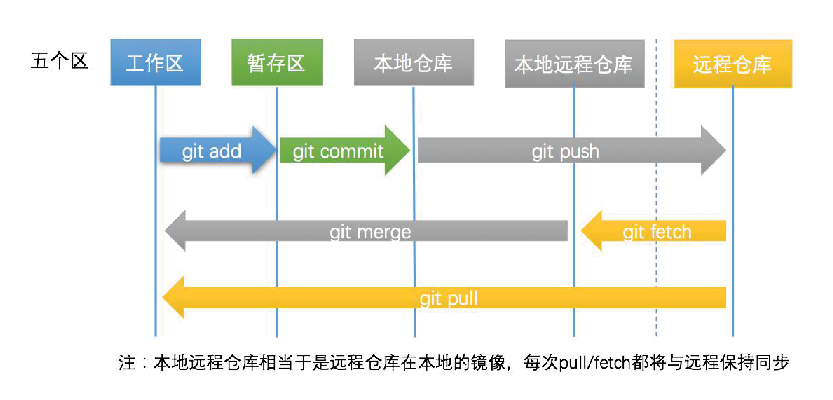
\includegraphics[width=1\textwidth]{1.eps}
  \caption{代码提交与工作流程图}
\end{figure}


\subsection{五种状态撤销更改图}

~


\begin{figure}[!h]
  \centering
  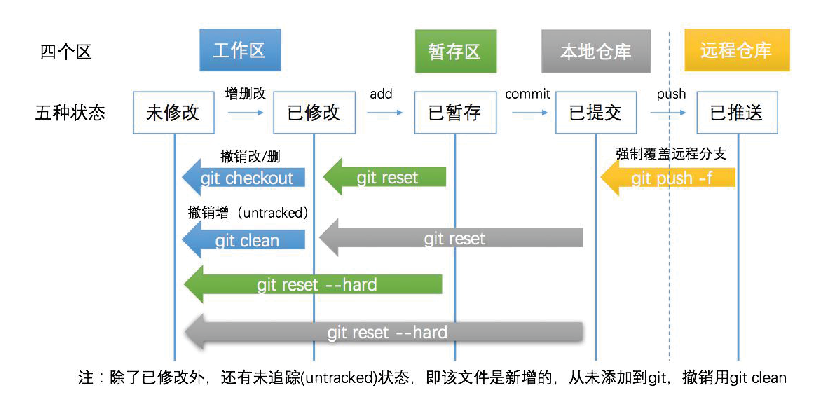
\includegraphics[width=1\textwidth]{2.eps}
  \caption{五种状态撤销更改图}
\end{figure}
\newpage
\section{创建版本库}
\subsection{初始化版本库}
\begin{lstlisting}
$git init
\end{lstlisting}

\subsection{添加文件到版本库(本地仓库)}
\begin{lstlisting}
$git add <files> or git add . (completely add)
$git commit -m <message>
\end{lstlisting}
~\\
~\\
~\\
\section{\textcolor{red}{\textbf{版本控制}}}

\subsection{\textbf{GIT RESET用法解析}}
\begin{lstlisting}
$git reset [--soft|--mixed|--hard] <commit>
\end{lstlisting}

\begin{figure}[!h]
  \centering
  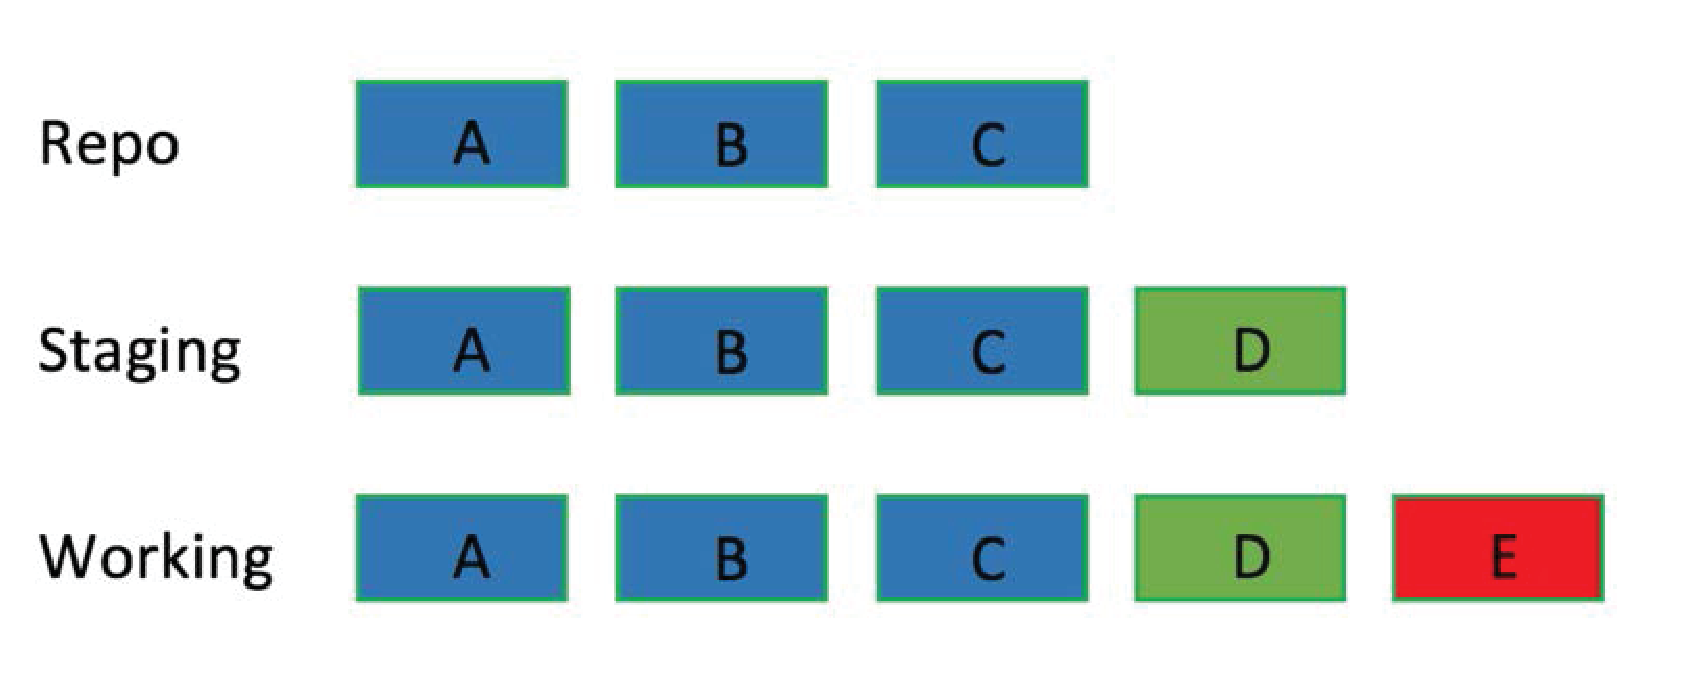
\includegraphics[width=0.9\textwidth]{GR1.eps}
  \caption{原始状态}
\end{figure}


\begin{lstlisting}
$git reset [--soft] <B commit>
\end{lstlisting}
\begin{figure}[!h]
  \centering
  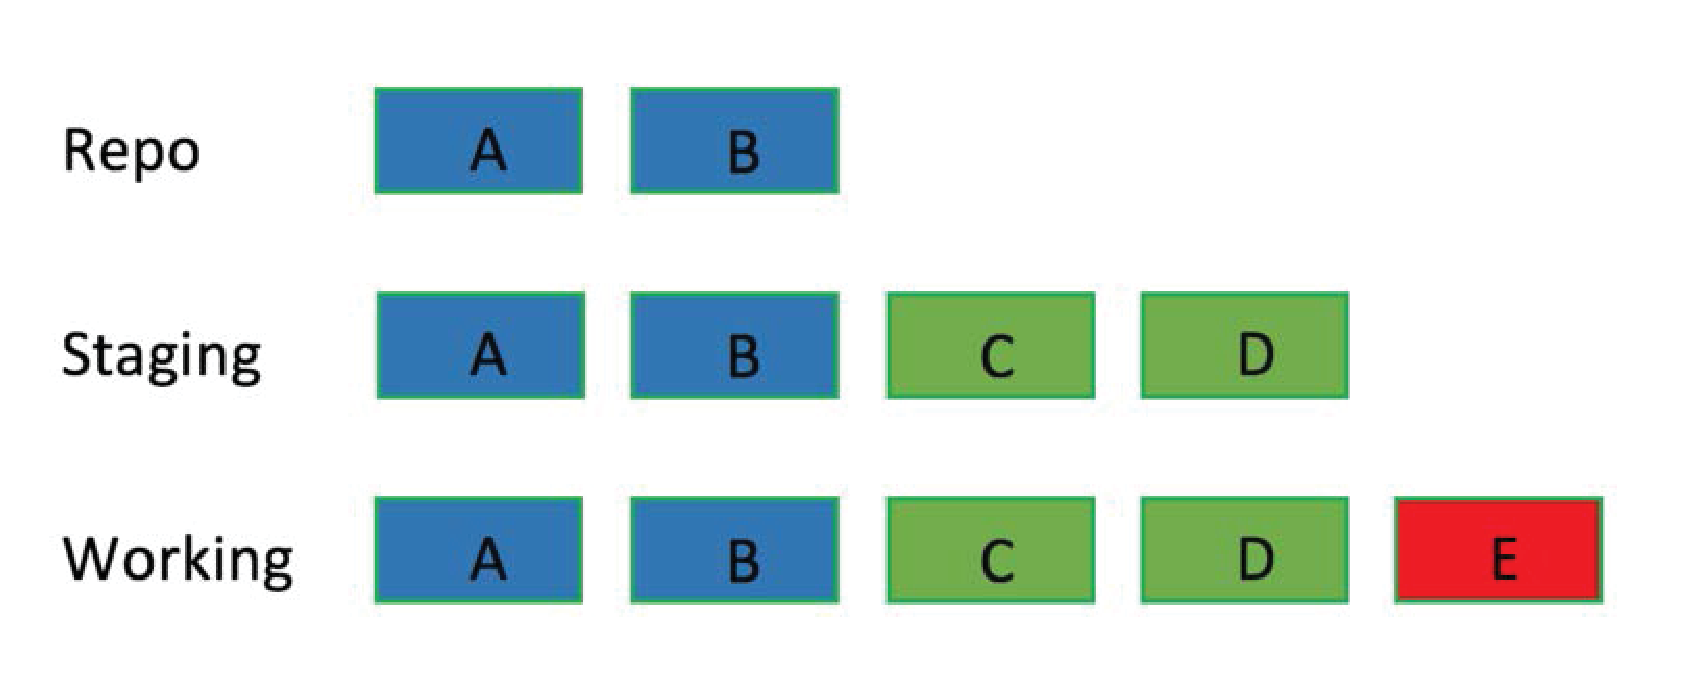
\includegraphics[width=0.9\textwidth]{GR2.eps}
  \caption{After git reset --soft B}
\end{figure}


\begin{lstlisting}
$git reset [--mixed] <B commit>
\end{lstlisting}
\begin{figure}[!h]
  \centering
  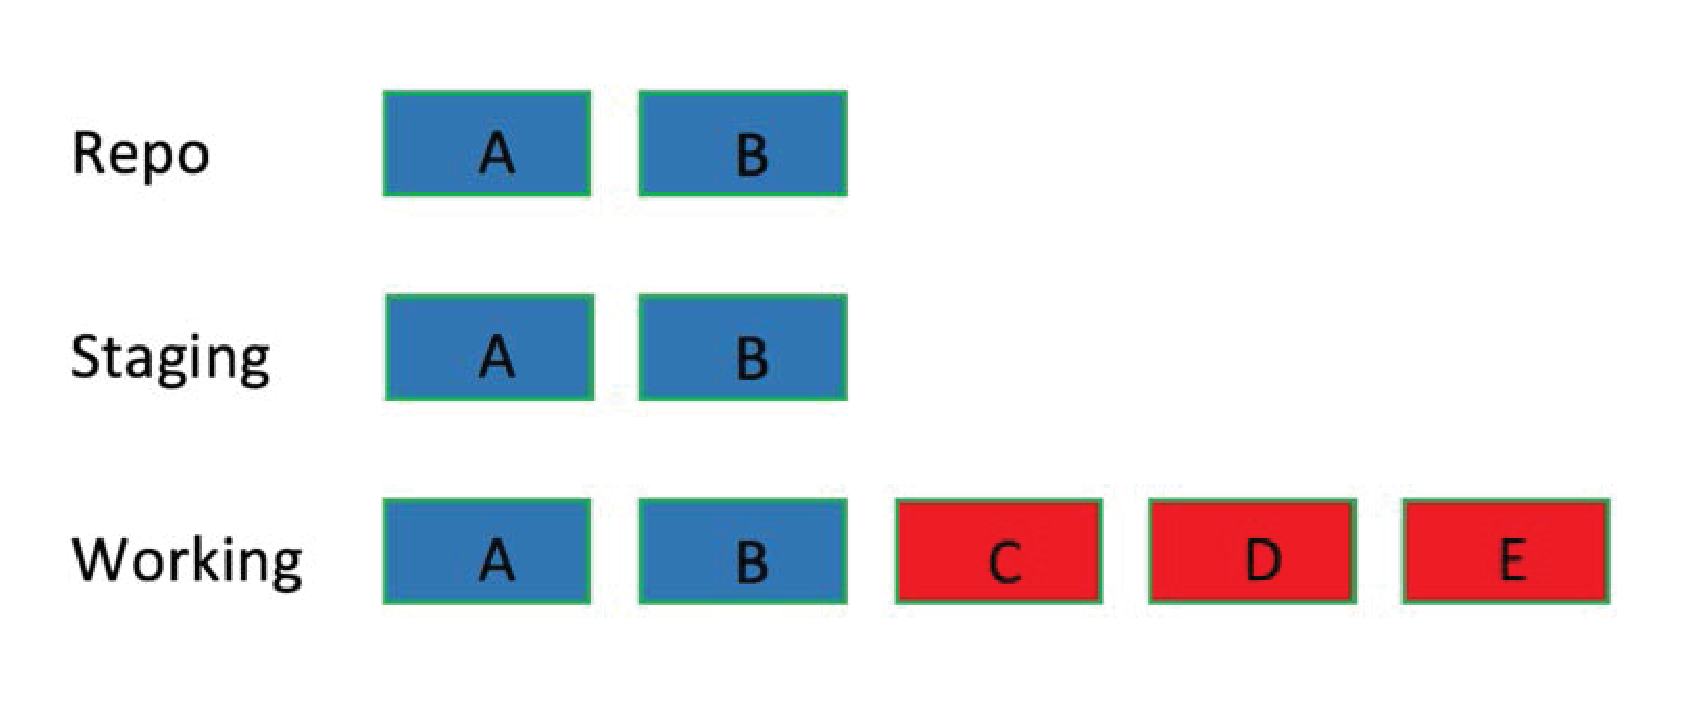
\includegraphics[width=0.9\textwidth]{GR3.eps}
  \caption{After git reset --mixed B}
\end{figure}


\begin{lstlisting}
$git reset [--hard] <B commit>
\end{lstlisting}
\begin{figure}[!h]
  \centering
  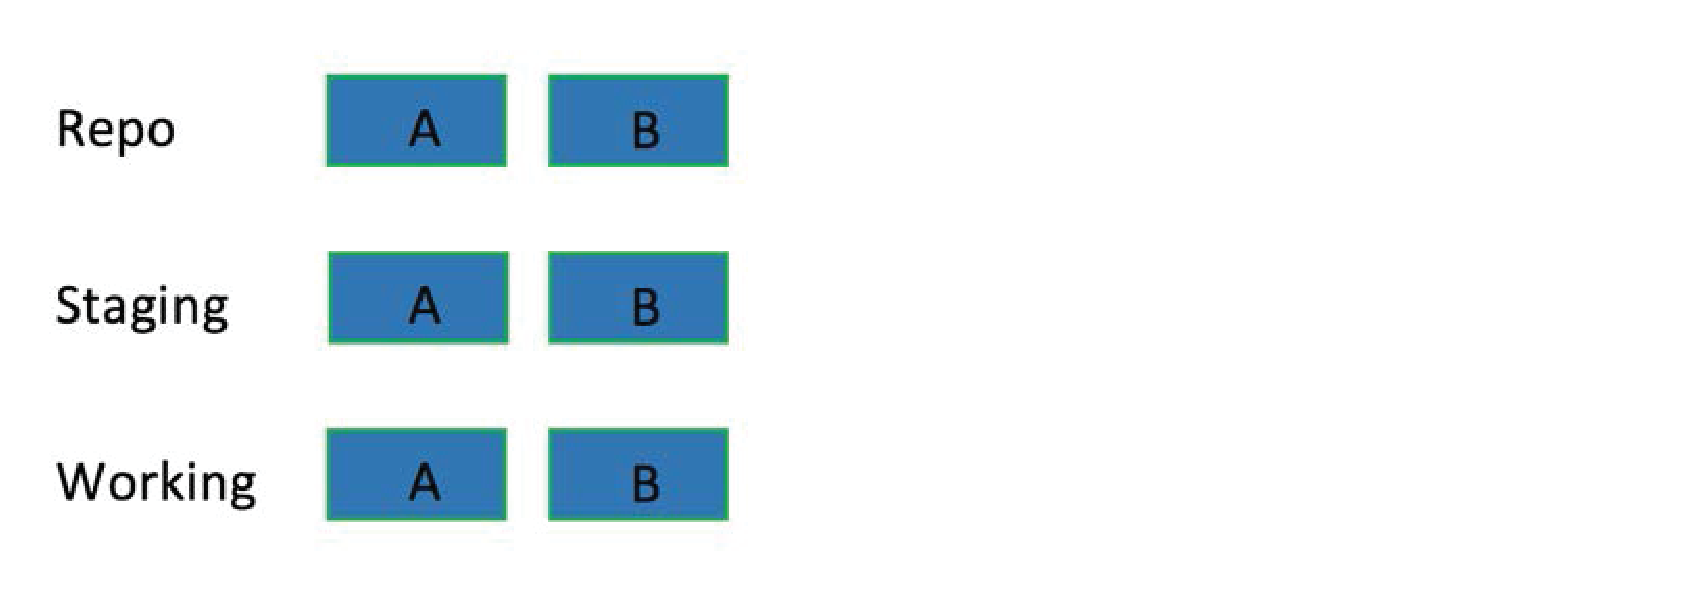
\includegraphics[width=0.9\textwidth]{GR4.eps}
  \caption{After git reset --hard B}
\end{figure}



\subsection{版本回退}
\subsubsection{查看提交历史}
\begin{lstlisting}
$git log --pretty=oneline --graph --all --decorate
\end{lstlisting}

\subsubsection{版本回退}
\begin{lstlisting}
$git reset --hard commit_id
\end{lstlisting}

\subsubsection{版本前置}
\begin{lstlisting}
$git reflog
$git reset --hard commit_id
\end{lstlisting}

\subsection{撤销修改}
\subsubsection{丢弃工作区的修改}
\begin{lstlisting}
$git checkout <files>
\end{lstlisting}

\subsubsection{丢弃已添加到暂存区的修改}
\begin{lstlisting}
$git reset HEAD <files>
$git checkout <files>
\end{lstlisting}

\subsection{删除文件}
\subsubsection{删除工作区文件}
\begin{lstlisting}
$git rm <files>
\end{lstlisting}

\subsubsection{确认删除则提交版本库}
\begin{lstlisting}
$git add .
$git commit -m <message>
\end{lstlisting}

\subsubsection{误删则暂存区替换工作区版本}
\begin{lstlisting}
$git checkout <files>
\end{lstlisting}

\section{远程仓库}
\subsection{添加远程库}
\begin{lstlisting}
$git remote add origin <URL>
\end{lstlisting}

\subsection{推送最新修改}
\begin{lstlisting}
$git push -u origin master (at first)
$git push
\end{lstlisting}

\subsection{从远程库克隆}
\begin{lstlisting}
$git clone <URL>
\end{lstlisting}

~\\
\section{\textcolor{red}{\textbf{分支管理}}}
\subsection{分支的管理与合并}
\subsubsection{查看分支}
\begin{lstlisting}
$git branch
\end{lstlisting}

\subsubsection{创建分支}
\begin{lstlisting}
$git branch <name>
\end{lstlisting}

\subsubsection{切换分支}
\begin{lstlisting}
$git checkout <name>
\end{lstlisting}

\subsubsection{创建+切换分支}
\begin{lstlisting}
$git checkout -b <name>
\end{lstlisting}

\subsubsection{合并某分支到当前分支}
\begin{lstlisting}
$git merge <name>
\end{lstlisting}

\subsubsection{删除分支}
\begin{lstlisting}
$git branch -d <name>
\end{lstlisting}

\subsection{修复bug 临时存储}
\begin{lstlisting}
$git stash
$git checkout <bug>
$git stash pop
\end{lstlisting}

\subsection{多人协作}
\subsubsection{查看远程库信息}
\begin{lstlisting}
$git remote -v
\end{lstlisting}

\subsubsection{本地推送分支}
\begin{lstlisting}
$git push origin branch-name  (if fail,git pull)
\end{lstlisting}

\subsubsection{本地创建和远程分支对应的分支}
\begin{lstlisting}
$git checkout -b branch-name origin/branch-name
\end{lstlisting}

\subsubsection{建立本地分支和远程分支的关联}
\begin{lstlisting}
$git branch --set-upstream branch-name origin/branch-name
\end{lstlisting}

\subsubsection{远程抓取分支}
\begin{lstlisting}
$git pull
\end{lstlisting}

\subsection{REBASE}
\begin{figure}[!h]
  \centering
  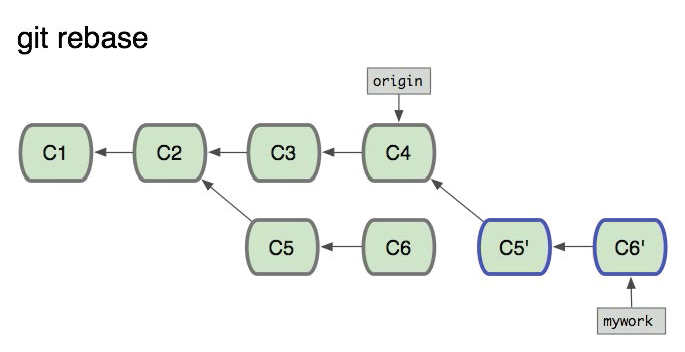
\includegraphics[width=0.8\textwidth]{3.eps}
  \caption{rebase}
\end{figure}

\begin{lstlisting}
$git rebase <branch name>
$fix conflict
$git add <files>
$git rebase --continue or git rebase --abort or git rebase --skip
\end{lstlisting}

\section{标签管理}
\subsection{创建标签}
\begin{lstlisting}
$git tag <tagname> or
$git tag -a <tagname> -m <message>
\end{lstlisting}

\subsection{查看所有标签}
\begin{lstlisting}
$git tag
\end{lstlisting}

\subsection{操作标签}
\subsubsection{推送本地标签到远程}
\begin{lstlisting}
$git push origin <tagname> (one tag)
$git push origin --tags (all tags)
\end{lstlisting}

\subsubsection{删除本地标签}
\begin{lstlisting}
$git tag -d <tagname>
\end{lstlisting}

\subsubsection{删除远程标签}
\begin{lstlisting}
$git push origin :refs/tags/<tagname>
\end{lstlisting} 